\documentclass[a4paper]{article}

\usepackage[english]{babel}
\usepackage[utf8]{inputenc}
\usepackage{amsmath}
\usepackage{graphicx}
\usepackage[colorinlistoftodos]{todonotes}

\title{Model-based Closed-loop Validation of Medical Devices}

\author{You}

\begin{document}
\maketitle

\begin{abstract}
Your abstract.
\end{abstract}

\section{Closed-loop Medical Devices}
\begin{figure}[t]
		\centering
		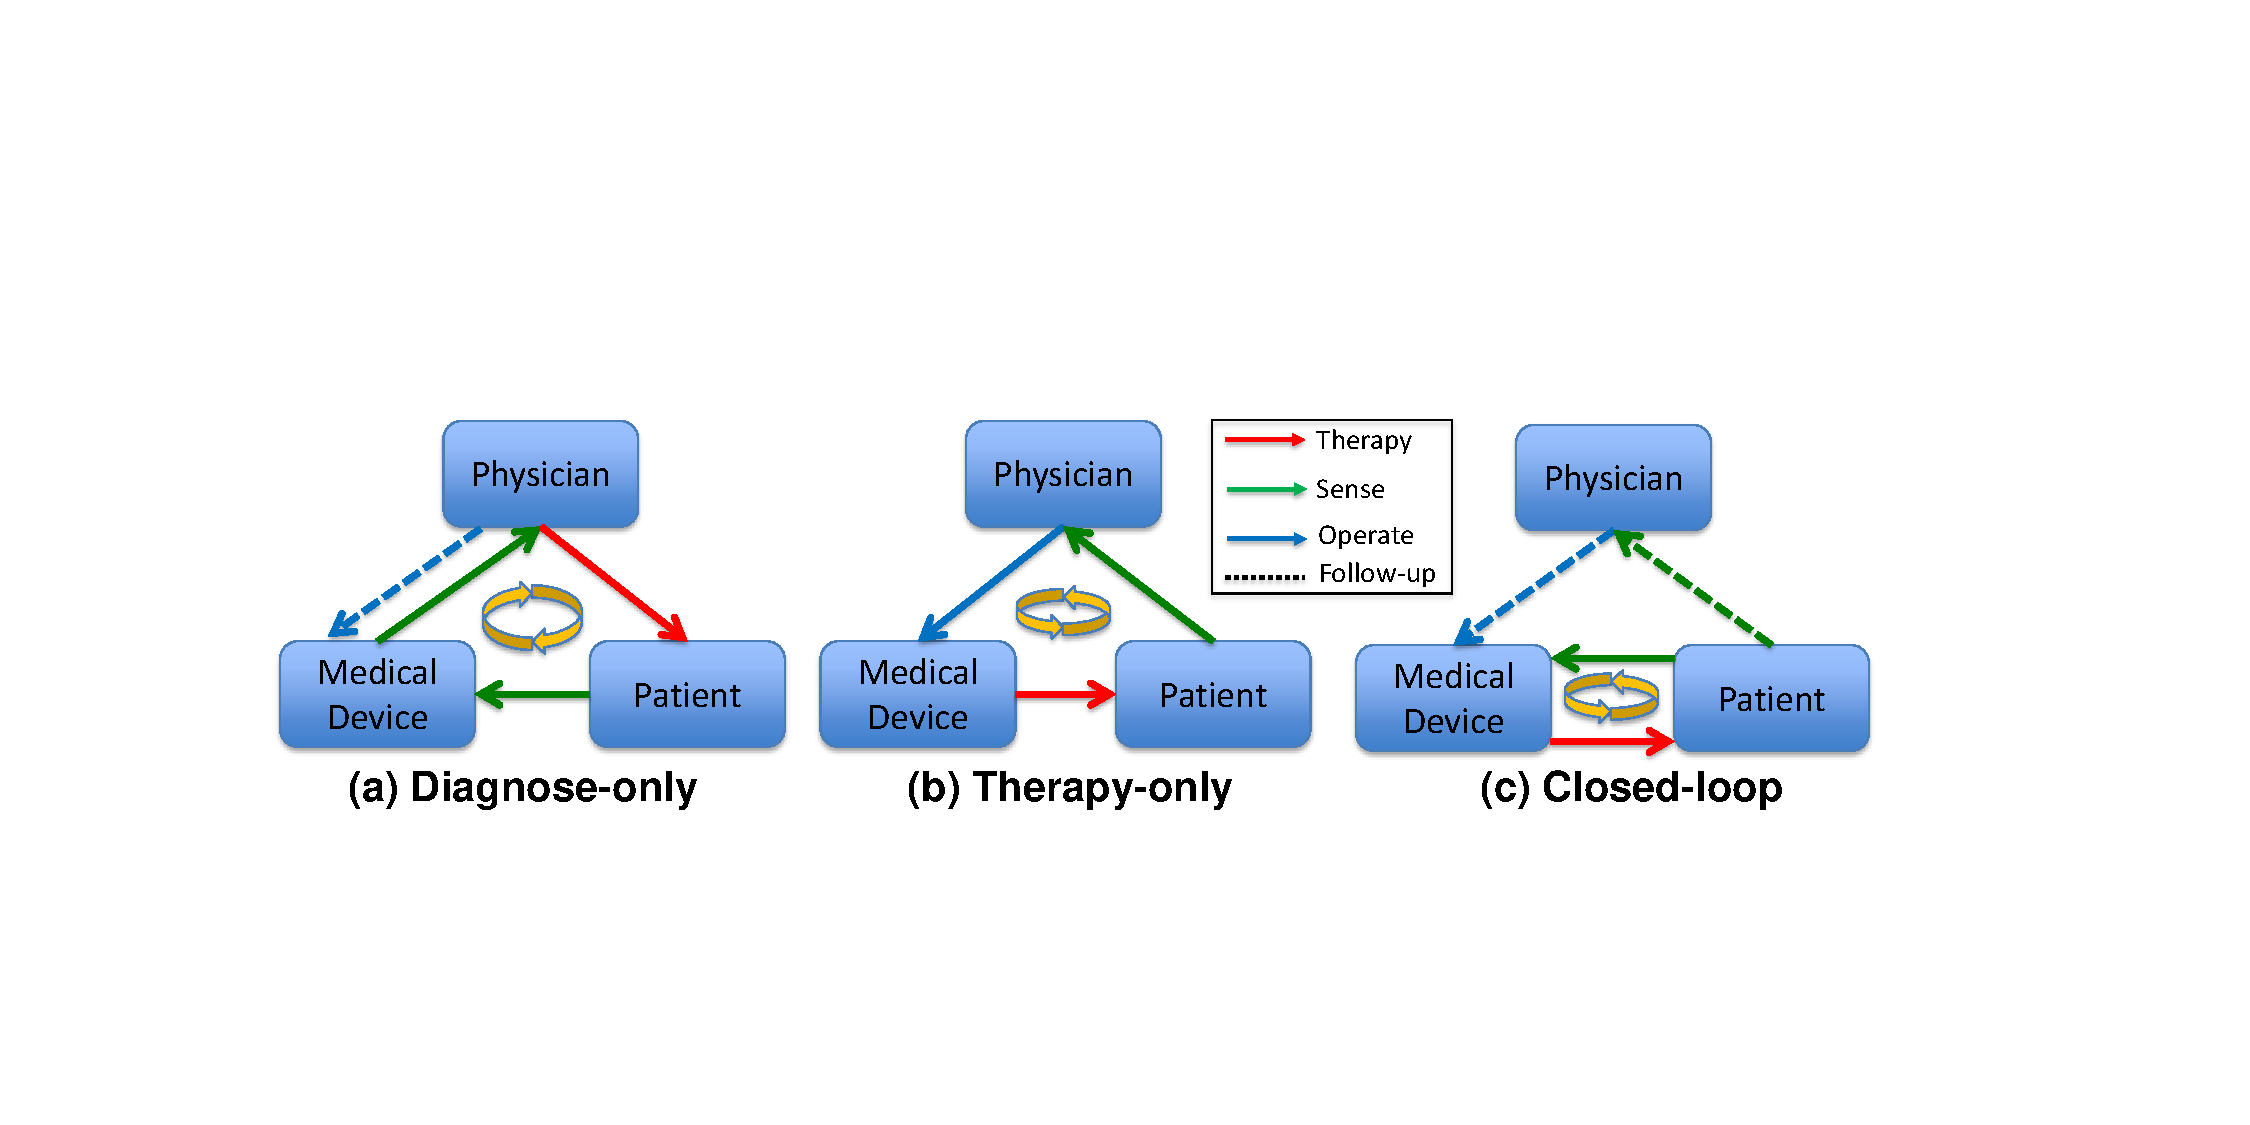
\includegraphics[width=\textwidth]{figs/closed-loop.pdf}
		\caption{\small Closing the Loop With the Patient}
		\label{fig:closed-loop}
\end{figure}
\begin{itemize}
	\item What are the differences between closed-loop medical devices vs. open-loop medical devices (Interact directly in closed-loop with physiology, With/without physician intervention)
	\item Example closed-loop medical devices (Pacemaker/ICD, deep brain stimulation, artificial pancreas, autonomous infusion pump)
	\item What are the challenges for closed-loop medical devices (interaction with physiology, limited capability, reliance on software)
	\item The need for closed-loop evaluation and the insufficiency of clinical trials as the only closed-loop evaluation method
\end{itemize}

\section{Computational Models for Physiological Behaviors}
Closed-loop validation of medical device
\begin{itemize}
	\item As example ,show list of different computational models of the heart (electrical, mechanical, anatomical)
	\item What are their applications? (understand mechanisms, predictions)
\end{itemize}

\section{Physiological Models for Closed-loop Evaluation of Closed-loop Medical Devices}
Model simulation results are accepted by FDA as safety evidence (Artificial pancreas)
\begin{itemize}
	\item Key characteristics for interaction with closed-loop medical devices (interface, distinguish conditions, interpretation of execution traces, identifiability)
	\item Why do aforementioned models not suitable for evaluating devices? (unnecessarily complex)
\end{itemize}

\section{Model-based Closed-loop Evaluation of Closed-loop Medical Devices}
Enable closed-loop validation earlier in the development process.
\begin{itemize}
	\item Two applications: Closed-loop Model checking and MBCT
	\item How do they fit into regulation framework

\end{itemize}

\subsection{Closed-loop Model Checking}
Can be used to identify known and unknown mechanisms that can induce hazards.
\begin{itemize}
	\item  Model considerations
	\item Device interface
	\item Coverage vs. Expressiveness
	\item Model refinement
\end{itemize}

\subsection{Model-based Clinical Trials}
Cover target population

\begin{itemize}
	\item Modeling considerations
	\item What is clinical trials and what can they achieve?
	\item What clinical trials cannot achieve? (\textbf{reproducibility}, large population)
	\item How can MBCT help?
\end{itemize}

\end{document}